\documentclass[handout]{beamer}
\usepackage{tikz}
\def\checkmark{\tikz\fill[scale=0.4](0,.35) -- (.25,0) -- (1,.7) -- (.25,.15) -- cycle;} 
\usepackage{pifont}
\newcommand{\xmark}{\ding{55}}
\usepackage{animate}
\usepackage{xcolor,cancel}

\usetheme{PaloAlto}
\title{Six lessons in inference}
\author[Ben]{Ben Lambert}
\date{\today}
\beamertemplatenavigationsymbolsempty
\setbeamertemplate{sidebar left}{}

\makeatletter
\newcommand\mathcircled[1]{%
	\mathpalette\@mathcircled{#1}%
}
\newcommand\@mathcircled[2]{%
	\tikz[baseline=(math.base)] \node[draw,circle,inner sep=1pt] (math) {$\m@th#1#2$};%
}

\begin{document}

\begin{frame}
\titlepage
\end{frame}

\begin{frame}
	\frametitle{Outline}
	\tableofcontents
\end{frame}

\section{What is inference?}

\frame{\tableofcontents[currentsection]}

\begin{frame}
	\frametitle{Data, $X$}
	
	\begin{figure}[ht]
		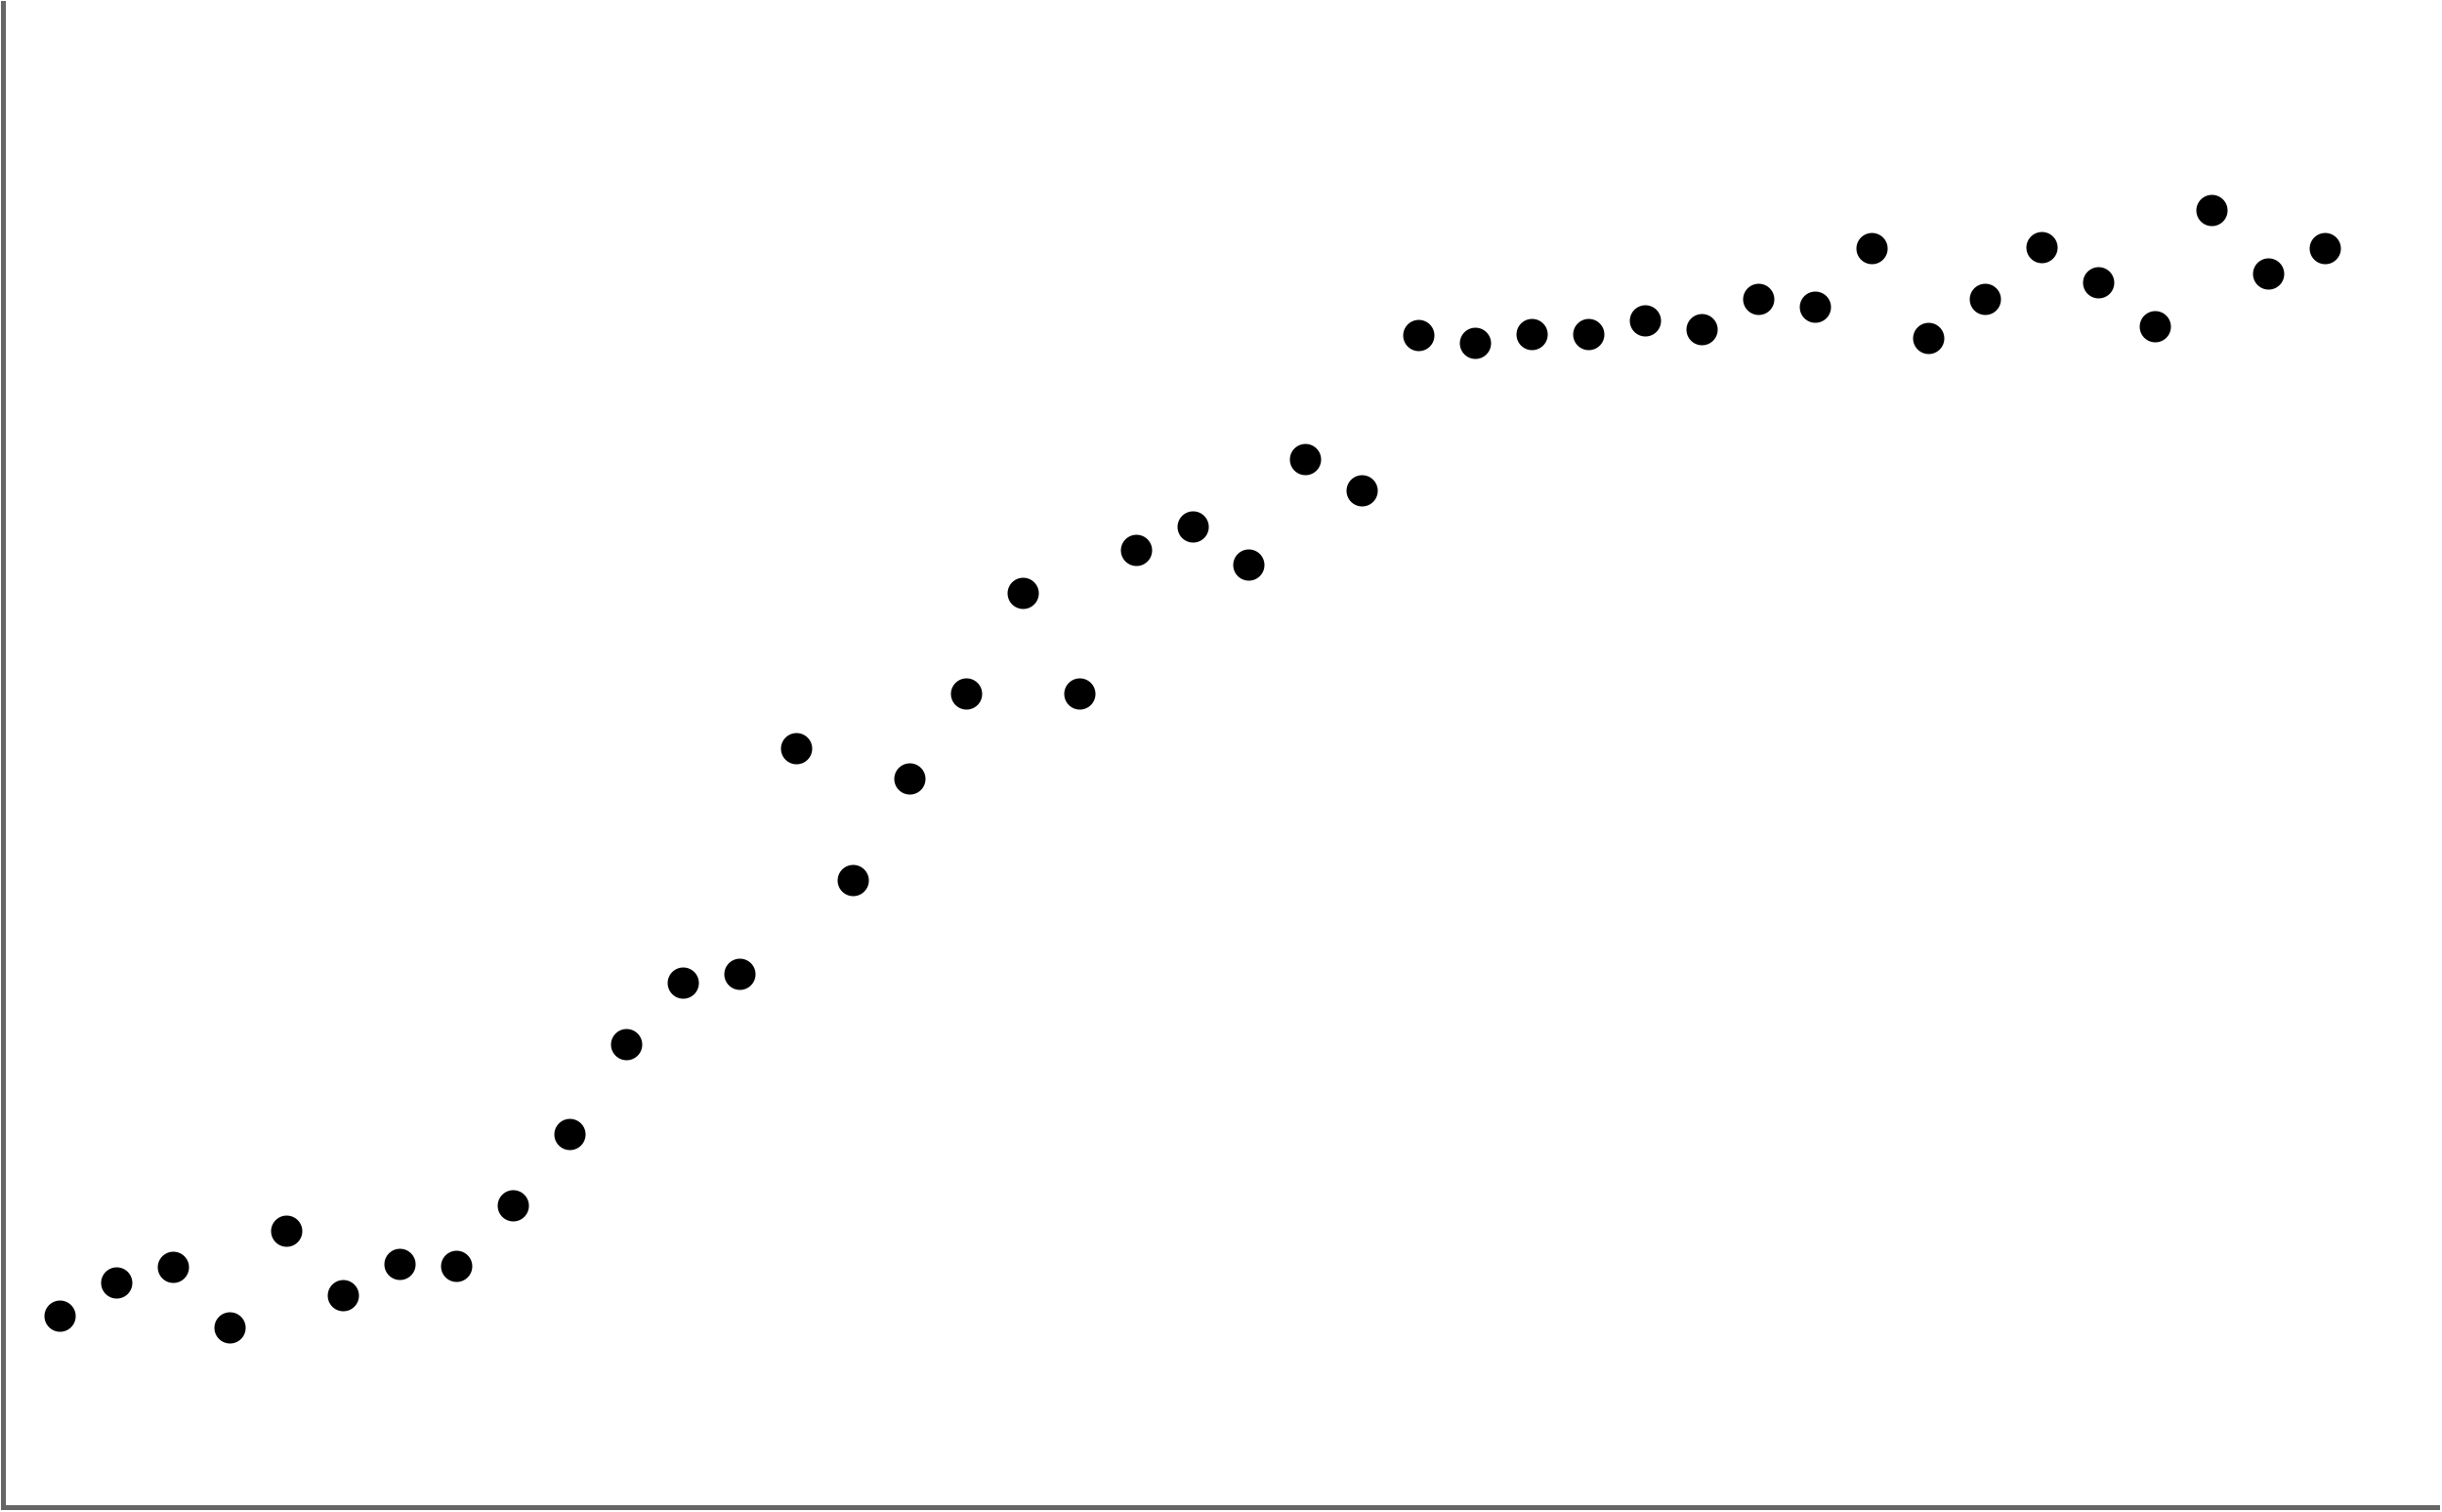
\includegraphics[width=1\textwidth]{./Animations/inference_data.png}
	\end{figure}
	
\end{frame}


\begin{frame}
	\frametitle{Example models, $f(\theta)$}
	
	\begin{figure}[t]
		\centerline{\animategraphics[width=1\textwidth,controls,buttonsize=1em,buttonfg=0.5]{2}{./Animations/inference_models_}{1}{10}}
	\end{figure}
\end{frame}

\begin{frame}
	\frametitle{Two types of inference}
	
	\begin{itemize}
		\item Optimisation: finds a single $\hat{\theta}$ that minimises some measure $||f(\hat{\theta})-X||$; 
		\item Distributional: finds a distribution $p(\theta)$ that represents a family of models that \textit{could} have generated data $X$, with varying weights.
	\end{itemize}
	
\end{frame}

\begin{frame}
	\frametitle{Aim of inference: optimisation}
	
	\begin{figure}[t]
		\centerline{\animategraphics[width=1\textwidth,controls,buttonsize=1em,buttonfg=0.5]{5}{./Animations/inference_optimisation_}{1}{60}}
	\end{figure}
\end{frame}

\begin{frame}
	\frametitle{Aim of inference: distribution of models}
	
		\begin{figure}[ht]
			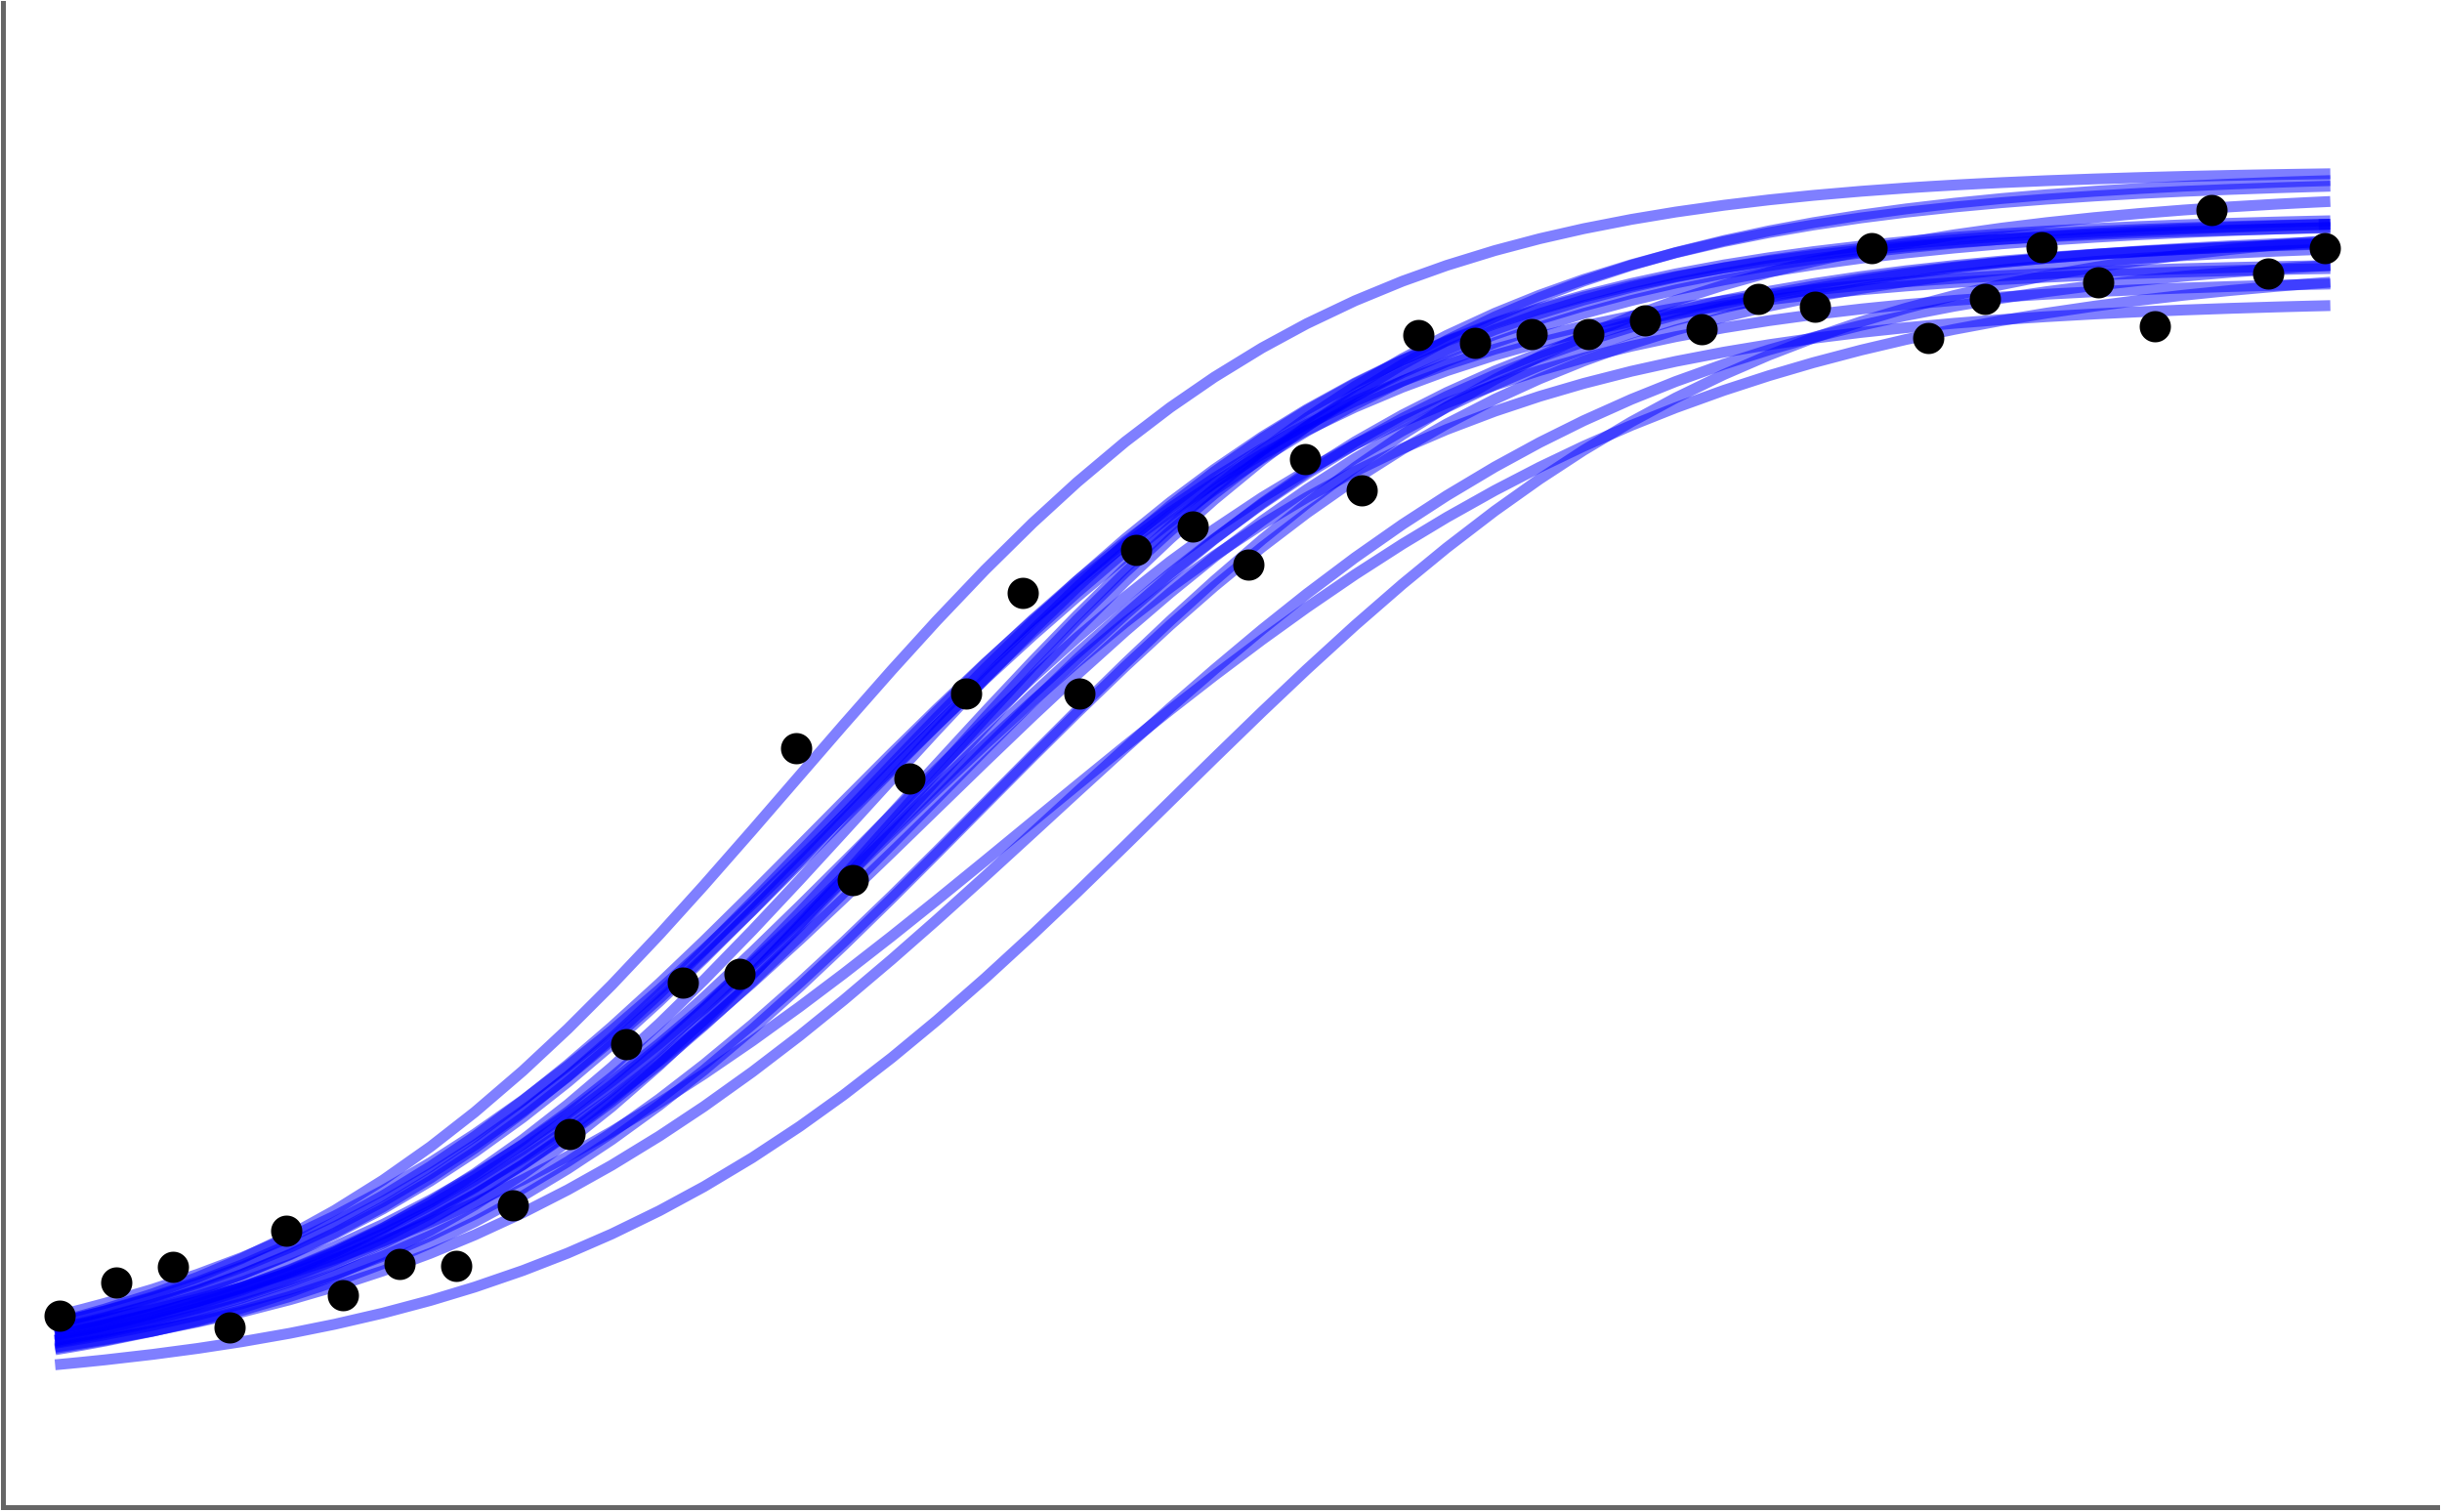
\includegraphics[width=1\textwidth]{./Animations/inference_sampling.png}
		\end{figure}
\end{frame}

\section{What is Bayesian inference?}

\frame{\tableofcontents[currentsection]}

\begin{frame}
	\frametitle{Bayes' rule}
	\begin{equation}
	p(\theta|X) = \frac{p(X|\theta)\times p(\theta)}{p(X)}
	\end{equation}
	
	But what do these terms mean?
\end{frame}

\begin{frame}
	\frametitle{Likelihood summary}
	
	\begin{equation}
	p(\theta|X) = \frac{\mathcircled{\color{blue}p(X|\theta)}\times p(\theta)}{p(X)}
	\end{equation}
	
	\begin{itemize}
		\item $\theta$ are parameters of sampling distribution.
		\item $X$ is data.
		\item $p(X|\theta)$ represents the \textit{likelihood}. 
		\item \textit{Not} a probability distribution because $\theta$ varies.
		\item Encapsulates many \textbf{subjective} judgements about analysis.
	\end{itemize}
	
\end{frame}

\begin{frame}
	\frametitle{Priors summary}
	\begin{equation}
	p(\theta|X) = \frac{p(X|\theta)\times \mathcircled{\color{blue}p(\theta)}}{p(X)}
	\end{equation}
	
	\begin{itemize}
		\item $p(\theta)$ represents the \textit{prior}. 
		\item A valid probability distribution.
		\item Similar to the likelihood; it is also subjective.
	\end{itemize}
\end{frame}

\begin{frame}
	\frametitle{Denominator summary}
	\begin{equation}
	p(\theta|X) = \frac{p(X|\theta)\times p(\theta)}{\mathcircled{\color{blue}p(X)}}
	\end{equation}
	
	\begin{itemize}
		\item $p(X)$ represents the \textit{denominator}.
		\item Two different interpretations:
		\begin{itemize}
			\item Before we collect $X$ $\implies$ \textbf{prior predictive distribution}.
			\item When we have data $X=2$ $\implies$ a normalising number known as the \textbf{evidence} or \textbf{marginal likelihood}.
		\end{itemize}
		\item Calculated from the numerator.
		\item Source of some difficulty of \textbf{exact} Bayesian inference (return to this later).
	\end{itemize}
\end{frame}

\begin{frame}
	\frametitle{Posteriors summary}
	\begin{equation}
	\mathcircled{\color{blue}p(\theta|X)} = \frac{p(X|\theta)\times p(\theta)}{p(X)}
	\end{equation}
	
	\begin{itemize}
		\item $p(\theta|X)$ represents the \textit{posterior}. 
		\item A valid probability distribution.
		\item Starting point for all further analysis in Bayesian inference.
	\end{itemize}
	
\end{frame}

\begin{frame}
	\frametitle{Intuition behind Bayesian analyses}
	Bayes' rule:
	
	\begin{equation}
	p(\theta|X) = \frac{p(X|\theta)\times p(\theta)}{p(X)}
	\end{equation}
	
	Tells us that:
	
	\begin{equation}
	p(\theta|X) \propto p(X|\theta)\times p(\theta)
	\end{equation}
	
	$\implies$ the posterior is a essentially a weighted (geometric) mean of the prior and likelihood.
	
\end{frame}

\begin{frame}
	\frametitle{Example problem: paternal discrepancy}
	
	\begin{itemize}
		\item<2-> \textbf{Paternal discrepancy} is the term given to a child who has a biological father different to their supposed biological father.
		\item<3-> \textbf{Question:} how common is it?
		\item<4-> \textbf{Answer:} a recent meta-analysis of studies of ``paternal discrepancy'' (PD) found a rate of $\sim 10\%$.
		\item<5-> Suppose we have data for a random sample of 10 children's presence/absence of PD.
	\end{itemize}
	
	\onslide<6-> \textbf{Aim:} infer the prevalence of PD in the population ($\theta$).
	
	\onslide<1->
	\begin{figure}[ht]
		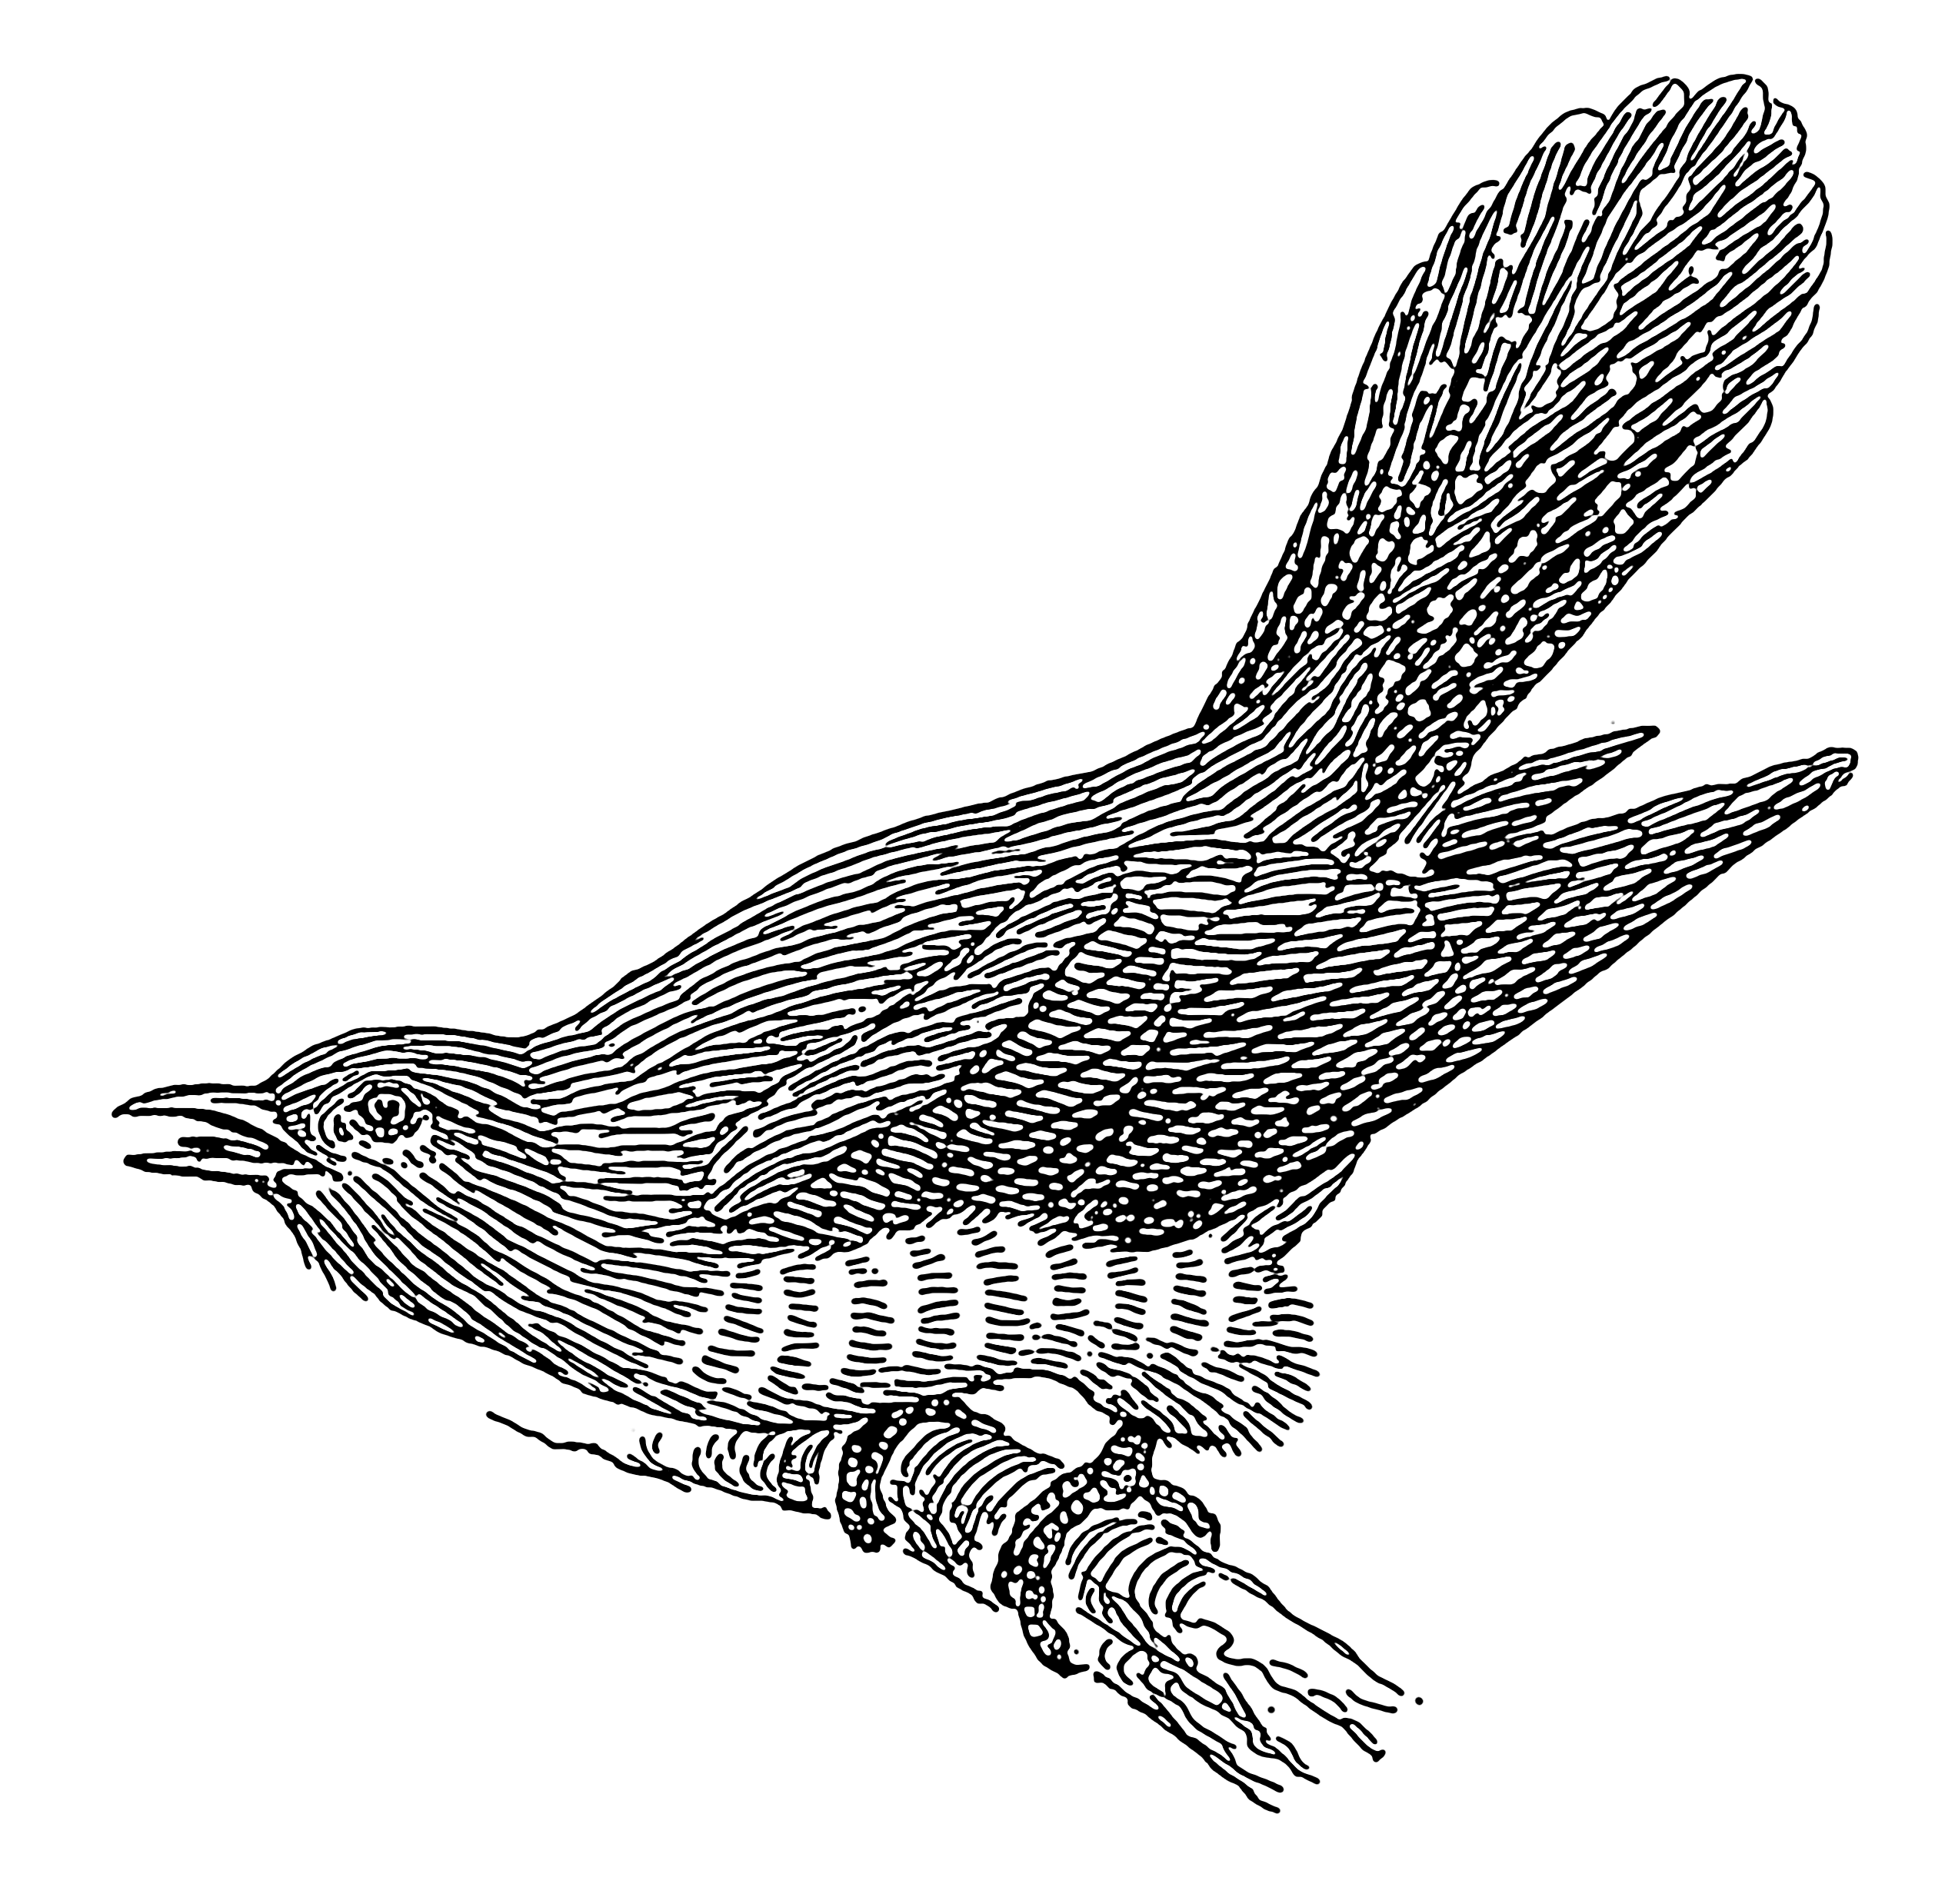
\includegraphics[width=0.5\textwidth]{./Animations/cuckoo.png}
	\end{figure}
	
\end{frame}

\begin{frame}
	\frametitle{Paternal discrepancy}
	Assume individual samples are:
	
	\begin{itemize}
		\item<2-> \textbf{Independent}.
		\item<3-> \textbf{Identically-distributed}.
	\end{itemize}
	
	\onslide<4-> 
	Since sample size is fixed at 10 $\implies$ binomial likelihood.
	
\end{frame}

\begin{frame}
	\frametitle{Intuition behind Bayesian analyses: PD rate again}
	Consider single sample of 10 children; 2 of which have PD.
	
	\begin{figure}[t]
		\centerline{\animategraphics[width=1\textwidth,controls,buttonsize=1em,buttonfg=0.5]{2}{./Animations/lec2_cuckooPriorToPosterior}{1}{37}}
	\end{figure}
\end{frame}

\begin{frame}
	\frametitle{Intuition behind Bayesian analyses: PD rate again}
	Now holding prior constant and varying proportion with PD.
	
	\begin{figure}[t]
		\centerline{\animategraphics[width=1\textwidth,controls,buttonsize=1em,buttonfg=0.5]{1}{./Animations/lec2_cuckooPriorToPosteriorLike}{1}{10}}
	\end{figure}
\end{frame}

\begin{frame}
	\frametitle{Intuition behind Bayesian analyses: PD rate again}
	Constant prior and proportion with PD (20\%); sample size$\uparrow$.
	
	\begin{figure}[t]
		\centerline{\animategraphics[width=1\textwidth,controls,buttonsize=1em,buttonfg=0.5]{2}{./Animations/lec2_cuckooPriorToPosteriorSample}{1}{20}}
	\end{figure}
\end{frame}

\begin{frame}
	\frametitle{An exception: zero priors (avoid these)}
	
	\begin{figure}
		\centerline{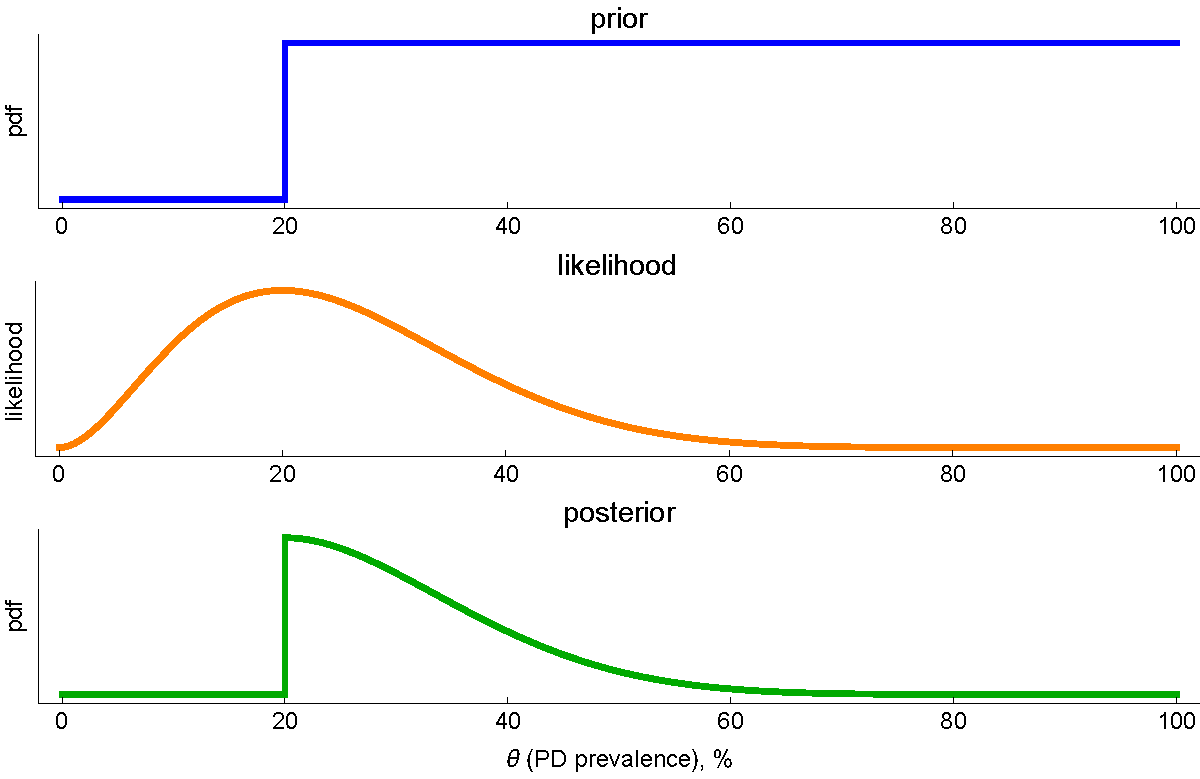
\includegraphics[width=1\textwidth]{./Animations/lec2_cuckooZeroPrior.pdf}}
	\end{figure}
	
\end{frame}

\section{The problem with exact Bayesian inference?}

\frame{\tableofcontents[currentsection]}

\begin{frame}
	\frametitle{The denominator revisited}
	\begin{equation}
	p(\theta|X=2) = \frac{p(X=2|\theta)\times p(\theta)}{\mathcircled{\color{blue}p(X=2)}}
	\end{equation}
	
	Where we suppose we have data $X=2$ out of a sample of 10 in our PD example.
	We obtain the denominator by averaging out all $\theta$ dependence. 
	This is equivalent to integrating across all $\theta$:
	
	\begin{equation}
	p(X=2) = \int\limits_{0}^{1} p(X=2|\theta)\times p(\theta) \mathrm{d}\theta
	\end{equation}
	
\end{frame}

\begin{frame}
	\frametitle{The denominator as an area}
	
	\begin{figure}
		\centerline{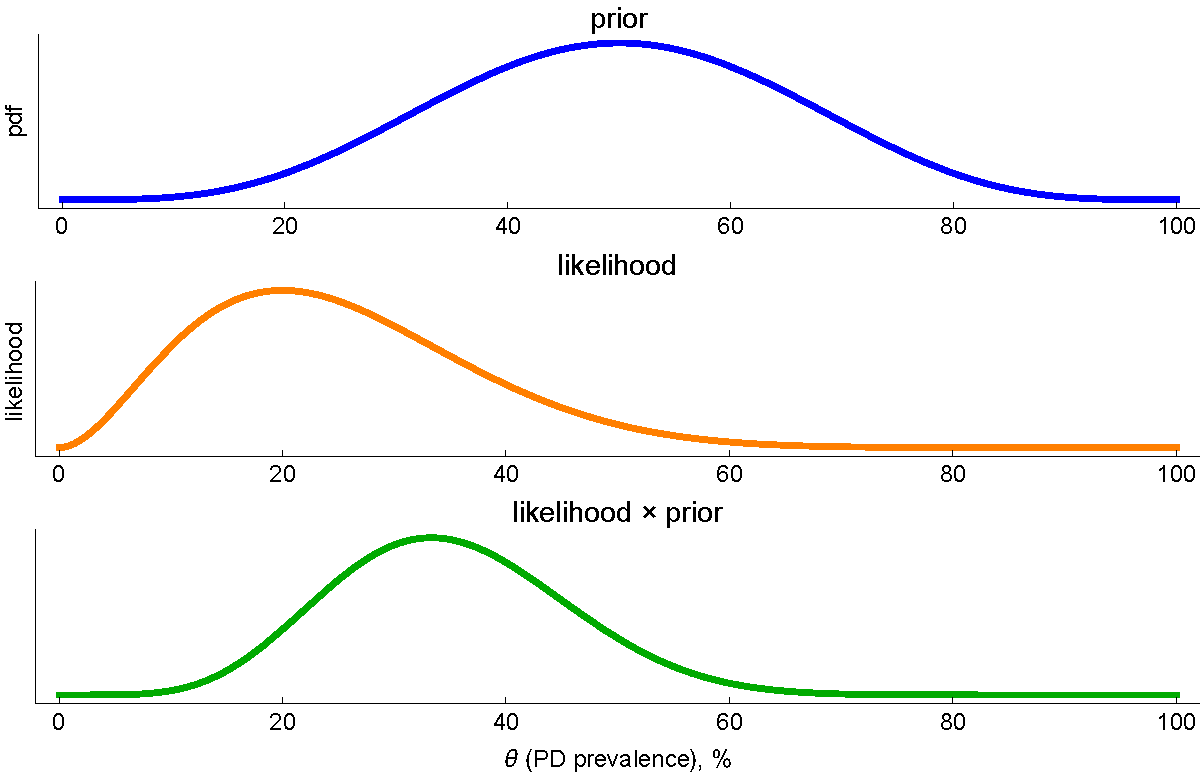
\includegraphics[width=1\textwidth]{./Animations/lec2_cuckooDenominator1.pdf}}
	\end{figure}
	
\end{frame}

\begin{frame}
	\frametitle{The denominator as an area}
	
	\begin{figure}
		\centerline{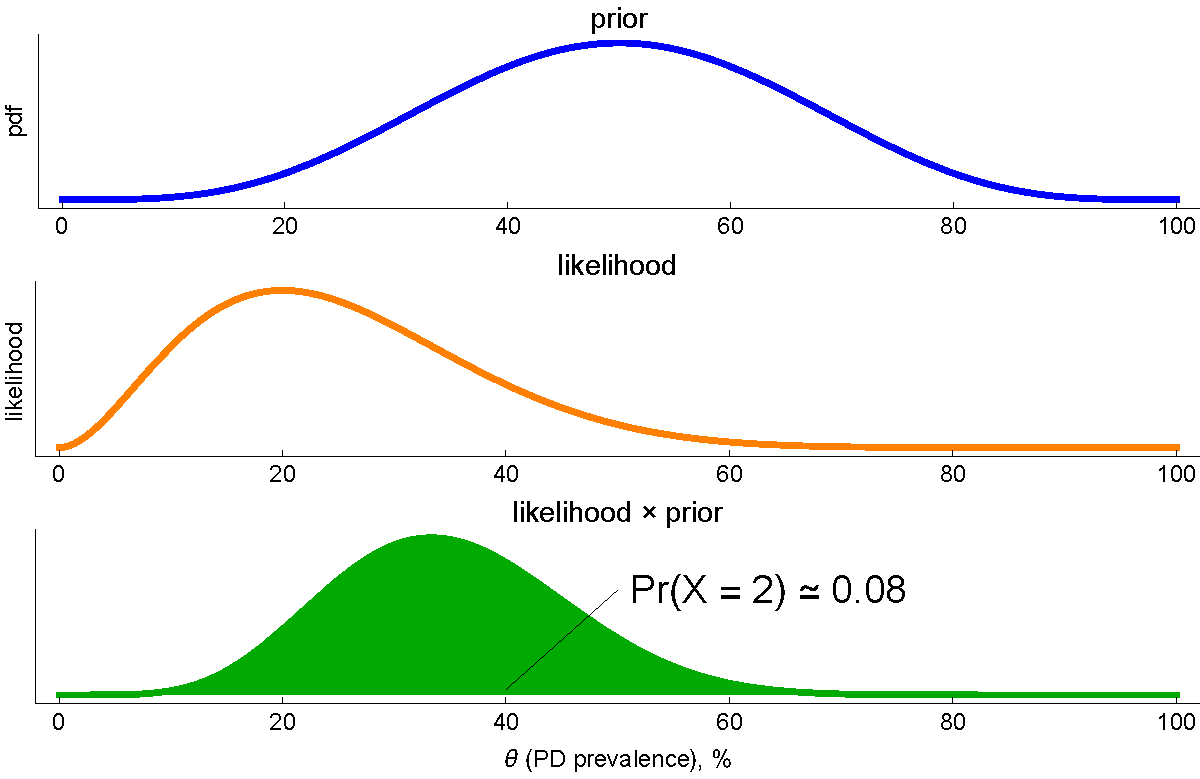
\includegraphics[width=1\textwidth]{./Animations/lec2_cuckooDenominator2.pdf}}
	\end{figure}
	
\end{frame}

\begin{frame}
	\frametitle{Calculating the denominator in 1 dimension}
For our PD example there is a single parameter $\theta \implies$
	

	\begin{equation}
	p(X=2) = \int\limits_{0}^{1} p(X=2|\theta)\times p(\theta) \mathrm{d}\theta
	\end{equation}
	
	This is equivalent to working out an \textbf{area} under a curve.
	
	\begin{figure}
		\centerline{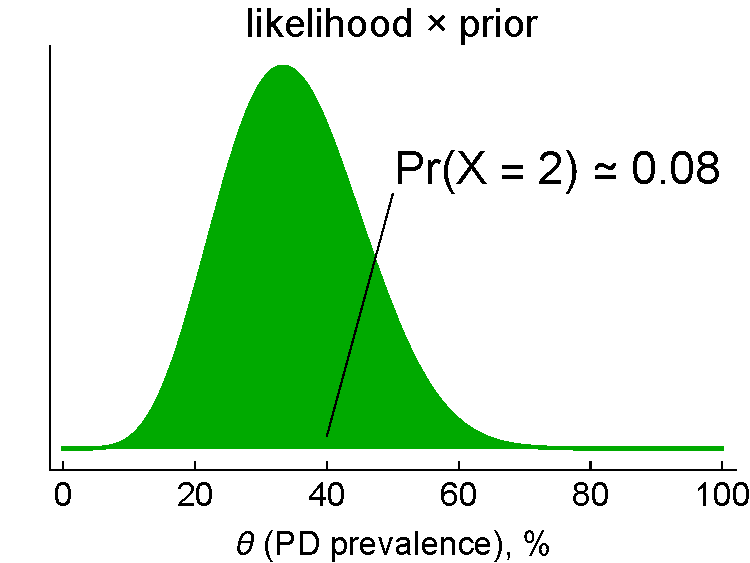
\includegraphics[width=0.6\textwidth]{./Animations/lec2_cuckooDenominator3.pdf}}
	\end{figure}
	
\end{frame}

\begin{frame}
	\frametitle{Calculating the denominator in 2 dimensions}
	If we considered a different model where there were two parameters $\theta_1\in(0,1),\; \theta_2\in(0,1)  \implies$:
	
	
	\begin{equation}
	p(X=2) = \int\limits_{0}^{1} \int\limits_{0}^{1} p(X=2|\theta_1,\theta_2)\times p(\theta_1,\theta_2) \mathrm{d}\theta_1 \mathrm{d}\theta_2 
	\end{equation}
	
	This is equivalent to working out a \textbf{volume} contained within a surface.
	
\end{frame}

\begin{frame}
	\frametitle{Calculating the denominator in $d$ dimensions}
	If we considered a different model where there were $d$ parameters $(\theta_1,...,\theta_d)$ all defined to lie between 0 and 1 $\implies$:
	
	\begin{equation}
	p(X=2) = \int\limits_{0}^{1} ... \int\limits_{0}^{1} p(X=2|\theta_1,...,\theta_d)\times p(\theta_1,...,\theta_d) \mathrm{d}\theta_1...\mathrm{d}\theta_d
	\end{equation}
	
	This is equivalent to working out a $(d+1)$-dimensional \textbf{volume} contained within a $d$-dimensional (hyper-surface)!
	
\end{frame}

\begin{frame}
	\frametitle{The difficult denominator}
	
	\begin{itemize}
		\item Calculating the denominator possible for $d < \sim 3$ using computers.
		\item Numerical quadrature and many other approximate schemes struggle for larger $d$.
		\item Many models have \textbf{thousands} of parameters.
	\end{itemize}
	
	$\implies$ side-step calculation of denominator by using sampling to understand the posterior.
	
\end{frame}

\section{What is sampling?}

\frame{\tableofcontents[currentsection]}

\begin{frame}
	\frametitle{Example of sampling: black box die}
	
	\begin{itemize}
		\item<2-> Black box containing a die with an \textbf{unknown} number of faces, and \textbf{weightings} towards sides. 
		\item<3-> Shake the box and view the number that lands face up through a viewing window.
		\item<4-> Note: an individual shake represents one \textbf{sample} from the probability distribution of the die.
	\end{itemize}
	
	\begin{figure}[ht]
		\centerline{\includegraphics[width=0.8\textwidth]{./Animations/dice1.pdf}}
	\end{figure}
	
\end{frame}

\begin{frame}
	\frametitle{Black box die: estimating mean}
	
	\begin{itemize}
		\item<2-> Question: How can we estimate the die's mean?
		\item<3-> Answer: shake it off! Then calculate the overall mean across all shakes.
	\end{itemize}
	
	\onslide<1->
	\begin{figure}[ht]
		\centerline{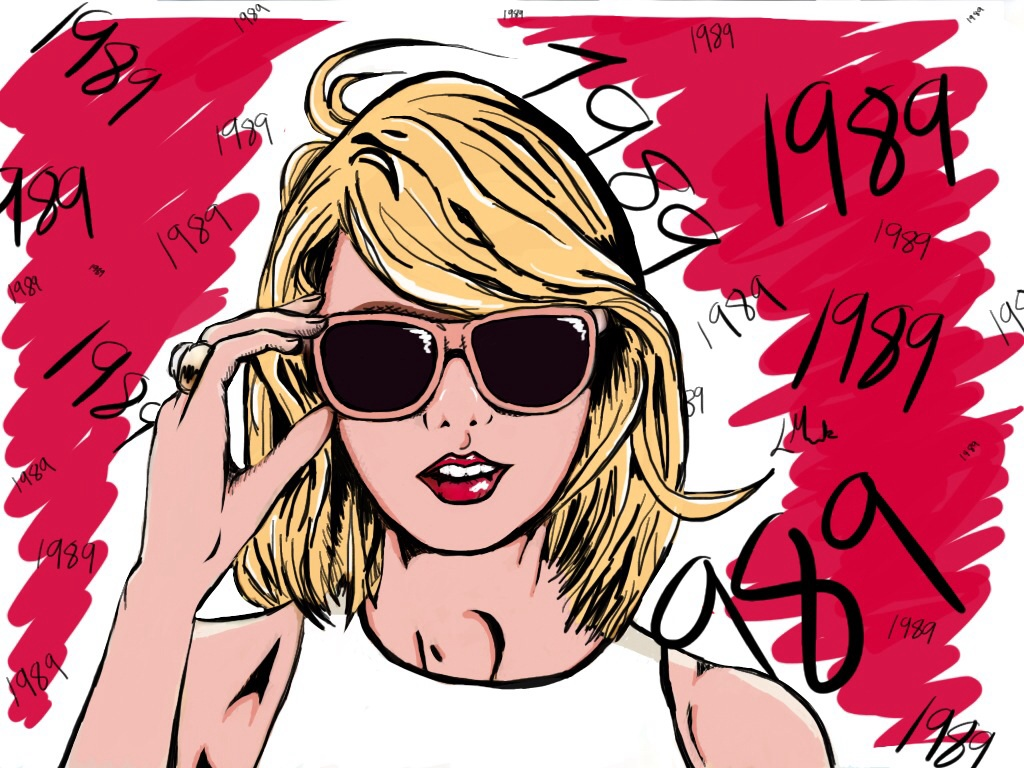
\includegraphics[width=1.0\textwidth]{./Animations/taylorSwift.jpg}}
	\end{figure}
	
\end{frame}


\begin{frame}
	\frametitle{Computational die in a box: results}
	
	\begin{figure}[t]
		\centerline{\animategraphics[width=0.9\textwidth,controls,buttonsize=1em,buttonfg=0.5]{8}{./Animations/lec3_dieRun}{1}{99}}
	\end{figure}
	
\end{frame}

\begin{frame}
	\frametitle{From a die to a posterior}
	
	We understood the completely unknown distribution of a die by sampling from it.
	
	\vspace{0.5cm}
	
	Markov chain Monte Carlo (MCMC) aims to do the same for the posterior.
	
\end{frame}

\begin{frame}
	\frametitle{MCMC basis}
	
	\begin{itemize}
		\item Flipping a coin was independent sampling;
		\item MCMC is a type of \textbf{dependent sampling}, which involves \textcolor{green}{accept} and \textcolor{red}{reject} steps.
	\end{itemize}
	
\end{frame}

\begin{frame}
	\frametitle{MCMC in action: aim to generate samples from this distribution}
		\begin{figure}[ht]
			\centerline{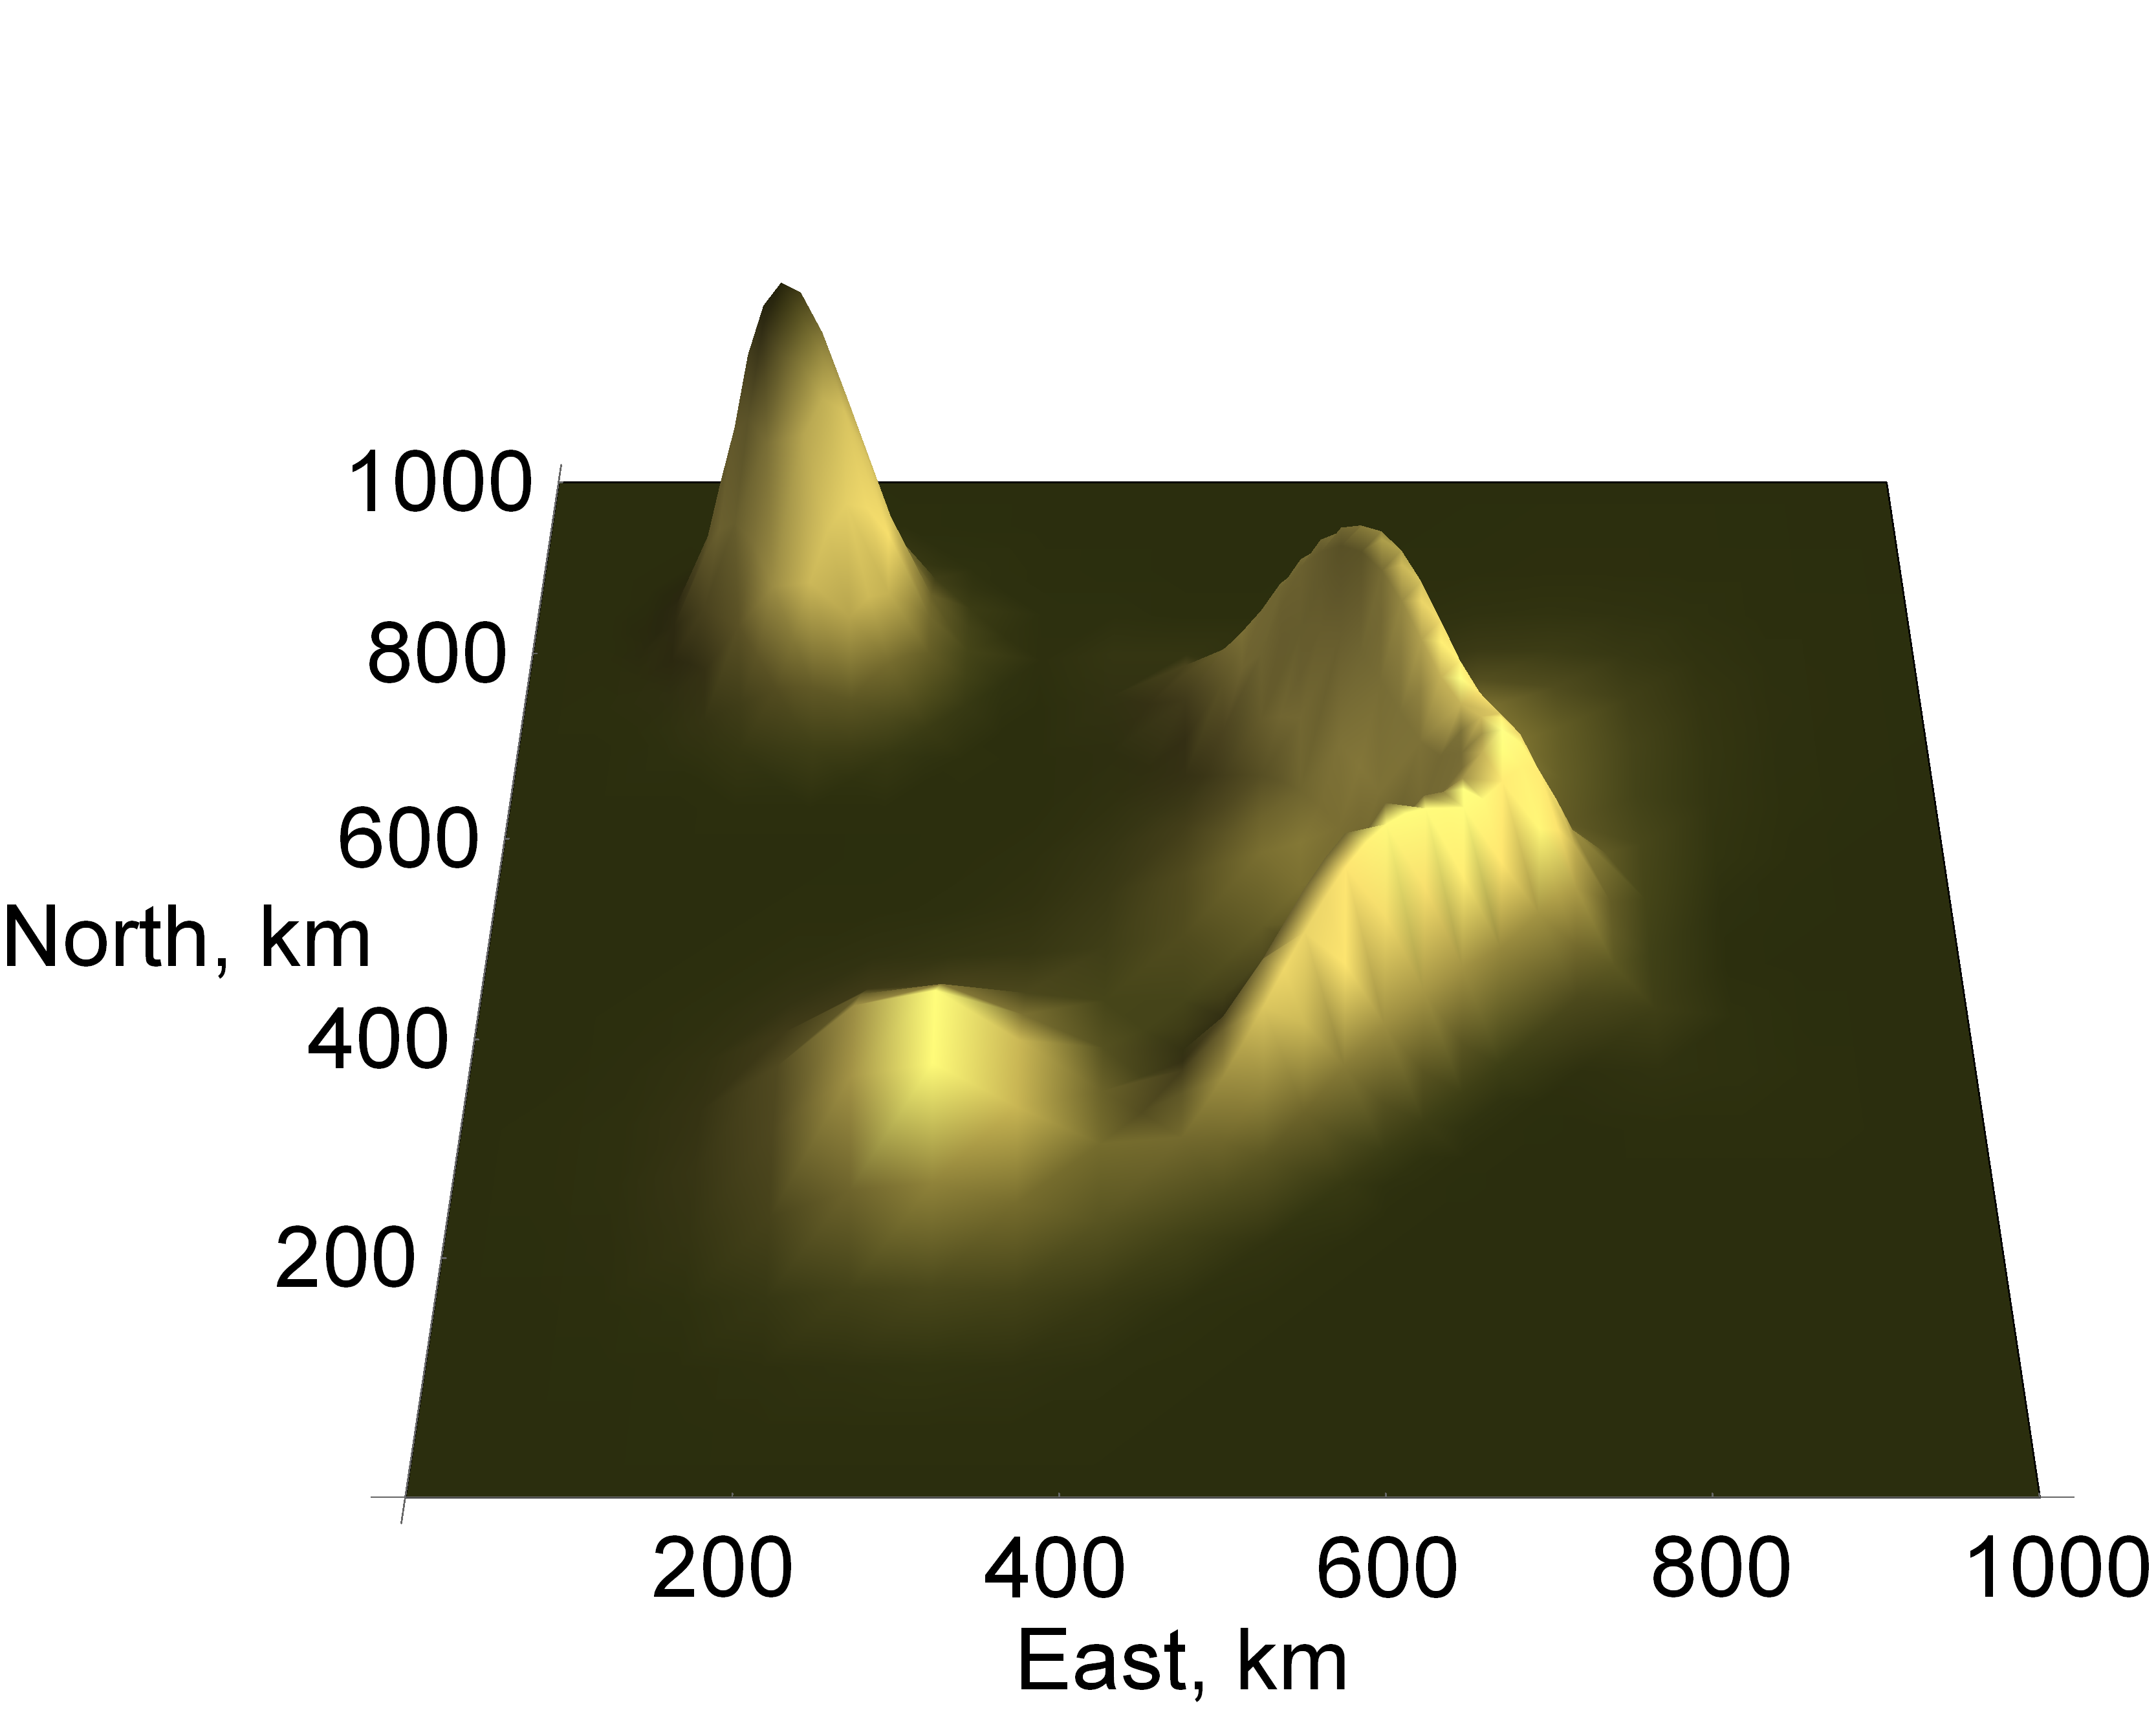
\includegraphics[width=0.8\textwidth]{./Animations/lec4_goldMiningActual.png}}
		\end{figure}
	\end{frame}
	
	\begin{frame}
		\frametitle{MCMC in action}
		\begin{figure}[t]
			\centerline{\animategraphics[width=0.75\textwidth,controls,buttonsize=1em,buttonfg=0.5]{2}{./Animations/lec4_goldMineAccept}{1}{101}}
		\end{figure}
		
	\end{frame}
	
	
	\begin{frame}
		\frametitle{Random Walk Metropolis in action}
		
		\begin{figure}[t]
			\centerline{\animategraphics[width=1\textwidth,controls,buttonsize=1em,buttonfg=0.5]{2}{./Animations/lec4_goldMining3D}{1}{48}}
		\end{figure}
		
	\end{frame}
	


\section{How to do inference for ODEs?}

\frame{\tableofcontents[currentsection]}

\begin{frame}
	\frametitle{ODE inference: postulate generative process for the model}
	
	Two parts:
	\begin{enumerate}
		\item Prior distribution governing likely values of parameters, $\theta_i \sim p(\theta)$;
		\item Sampling distribution which explains deviations from model predictions to observed data, $X_i\sim p(X|\theta_i)$.
	\end{enumerate}
	
	$\implies$ a posterior, $p(\theta|X)$ that summarises all uncertainty of parameter values.
	
	\vspace{0.5cm}
	
	But, how do we write down a sampling distribution for an ODE model?
	
\end{frame}


\begin{frame}
	\frametitle{ODEs: forward model}

	
	\begin{equation}
	\frac{d y(t)}{dt} = f(y, t; \theta).
	\end{equation}
	
	\begin{figure}
		\centerline{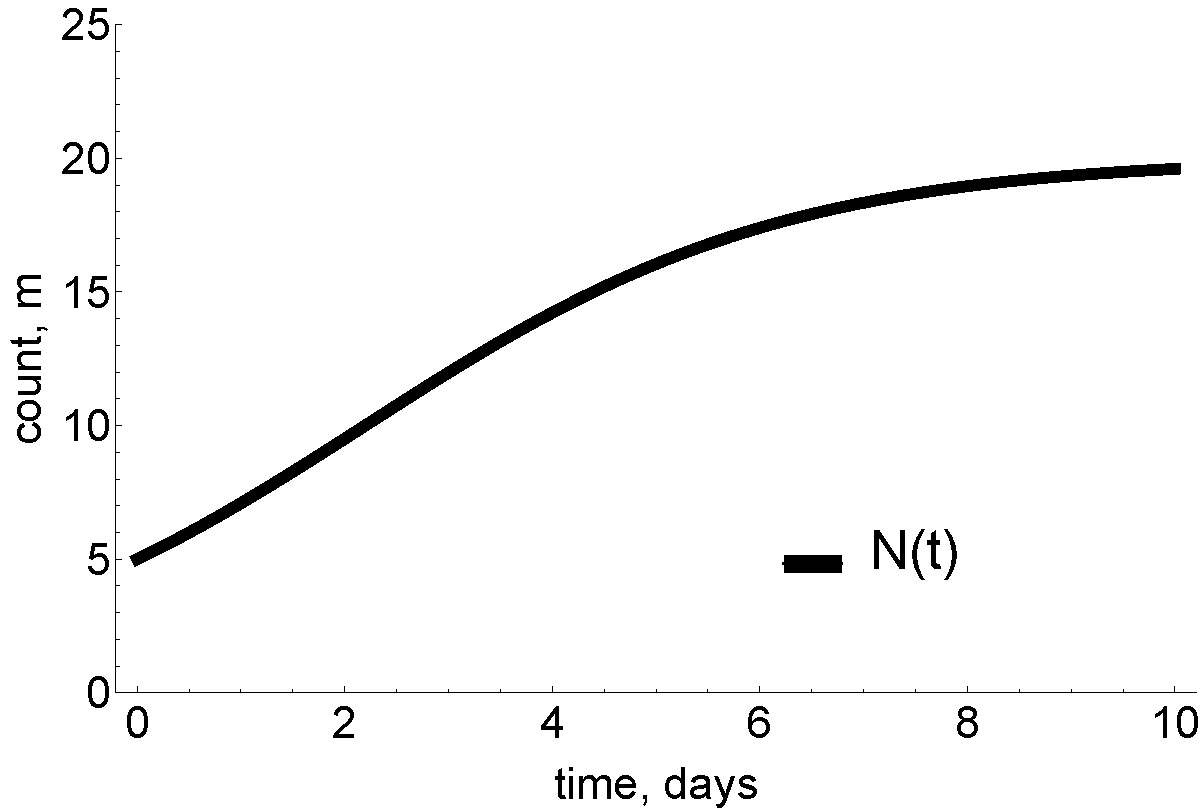
\includegraphics[width=0.7\textwidth]{./Figures/lec7_odeSingleBulding1.pdf}}
	\end{figure}
	
\end{frame}

\begin{frame}
	\frametitle{ODEs: noise model}
	
	
	\begin{equation}
	y^*(t) \stackrel{i.i.d.}{\sim} \mathcal{N}(y(t;\theta), \sigma).
	\end{equation}
	
	\begin{figure}
		\centerline{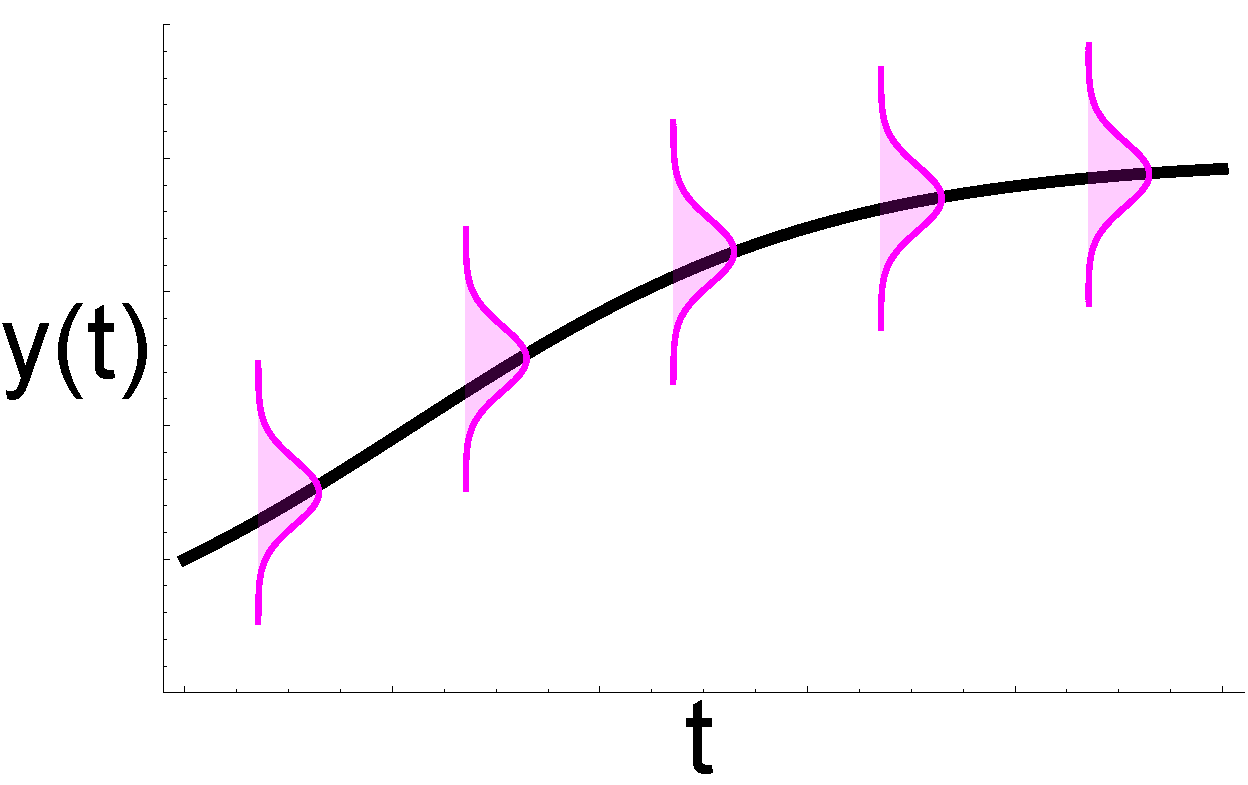
\includegraphics[width=0.7\textwidth]{./Figures/lec7_odeSingleBulding2.pdf}}
	\end{figure}
	
\end{frame}

\begin{frame}
	\frametitle{ODEs: data}
	
	\begin{equation}
	\mathcal{L} = \prod_{i=1}^{S} \mathcal{N}(y^*(t_i)| y(t_i;\theta), \sigma).
	\end{equation}
	
	\begin{figure}
		\centerline{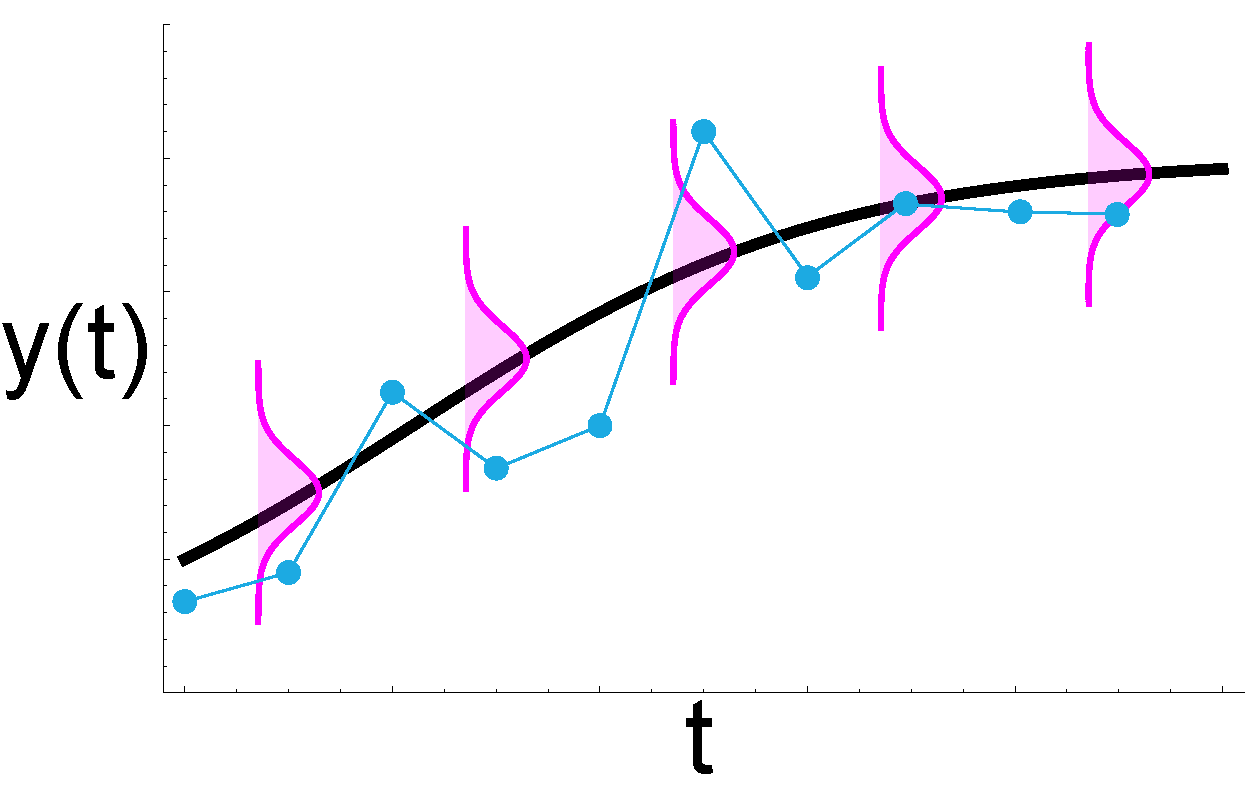
\includegraphics[width=0.7\textwidth]{./Figures/lec7_odeSingleBulding2_data.pdf}}
	\end{figure}
	
\end{frame}

\section{How to do practical inference?}

\frame{\tableofcontents[currentsection]}

\begin{frame}
	\frametitle{How to fit model to data?}
	
	\begin{figure}
		\centerline{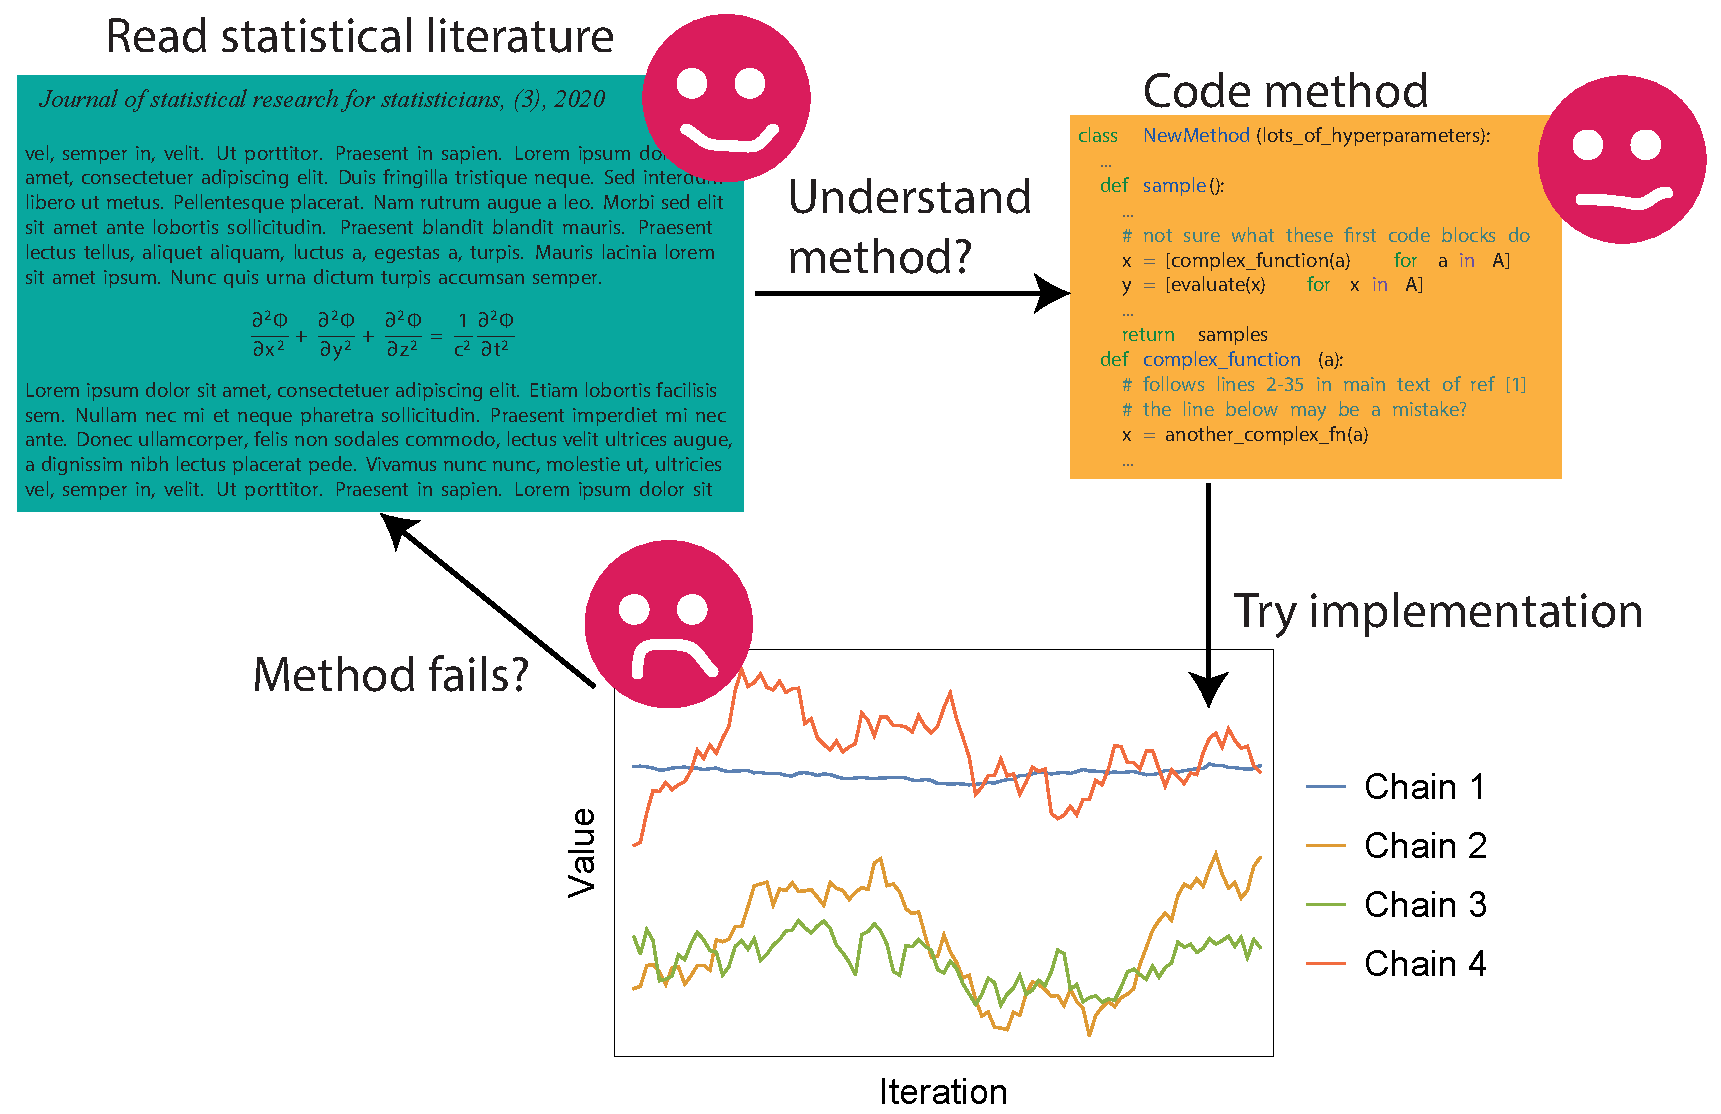
\includegraphics[width=1\textwidth]{./Figures/student_cycle.pdf}}
	\end{figure}
	
\end{frame}


\begin{frame}
\frametitle{To avoid misery: use Pints}

Pints: \textbf{P}robabilistic \textbf{I}nference for \textbf{N}oisy \textbf{T}ime \textbf{S}eries, which covers two broad categories of inference methods:

\begin{itemize}
	\item Optimisation: single set of parameters returned;
	\item Sampling: many sets returned.
\end{itemize}

It's an open-source Python library available on Github.

\end{frame}

\begin{frame}
\frametitle{Pints roadmap: samplers}

\begin{figure}
	\centerline{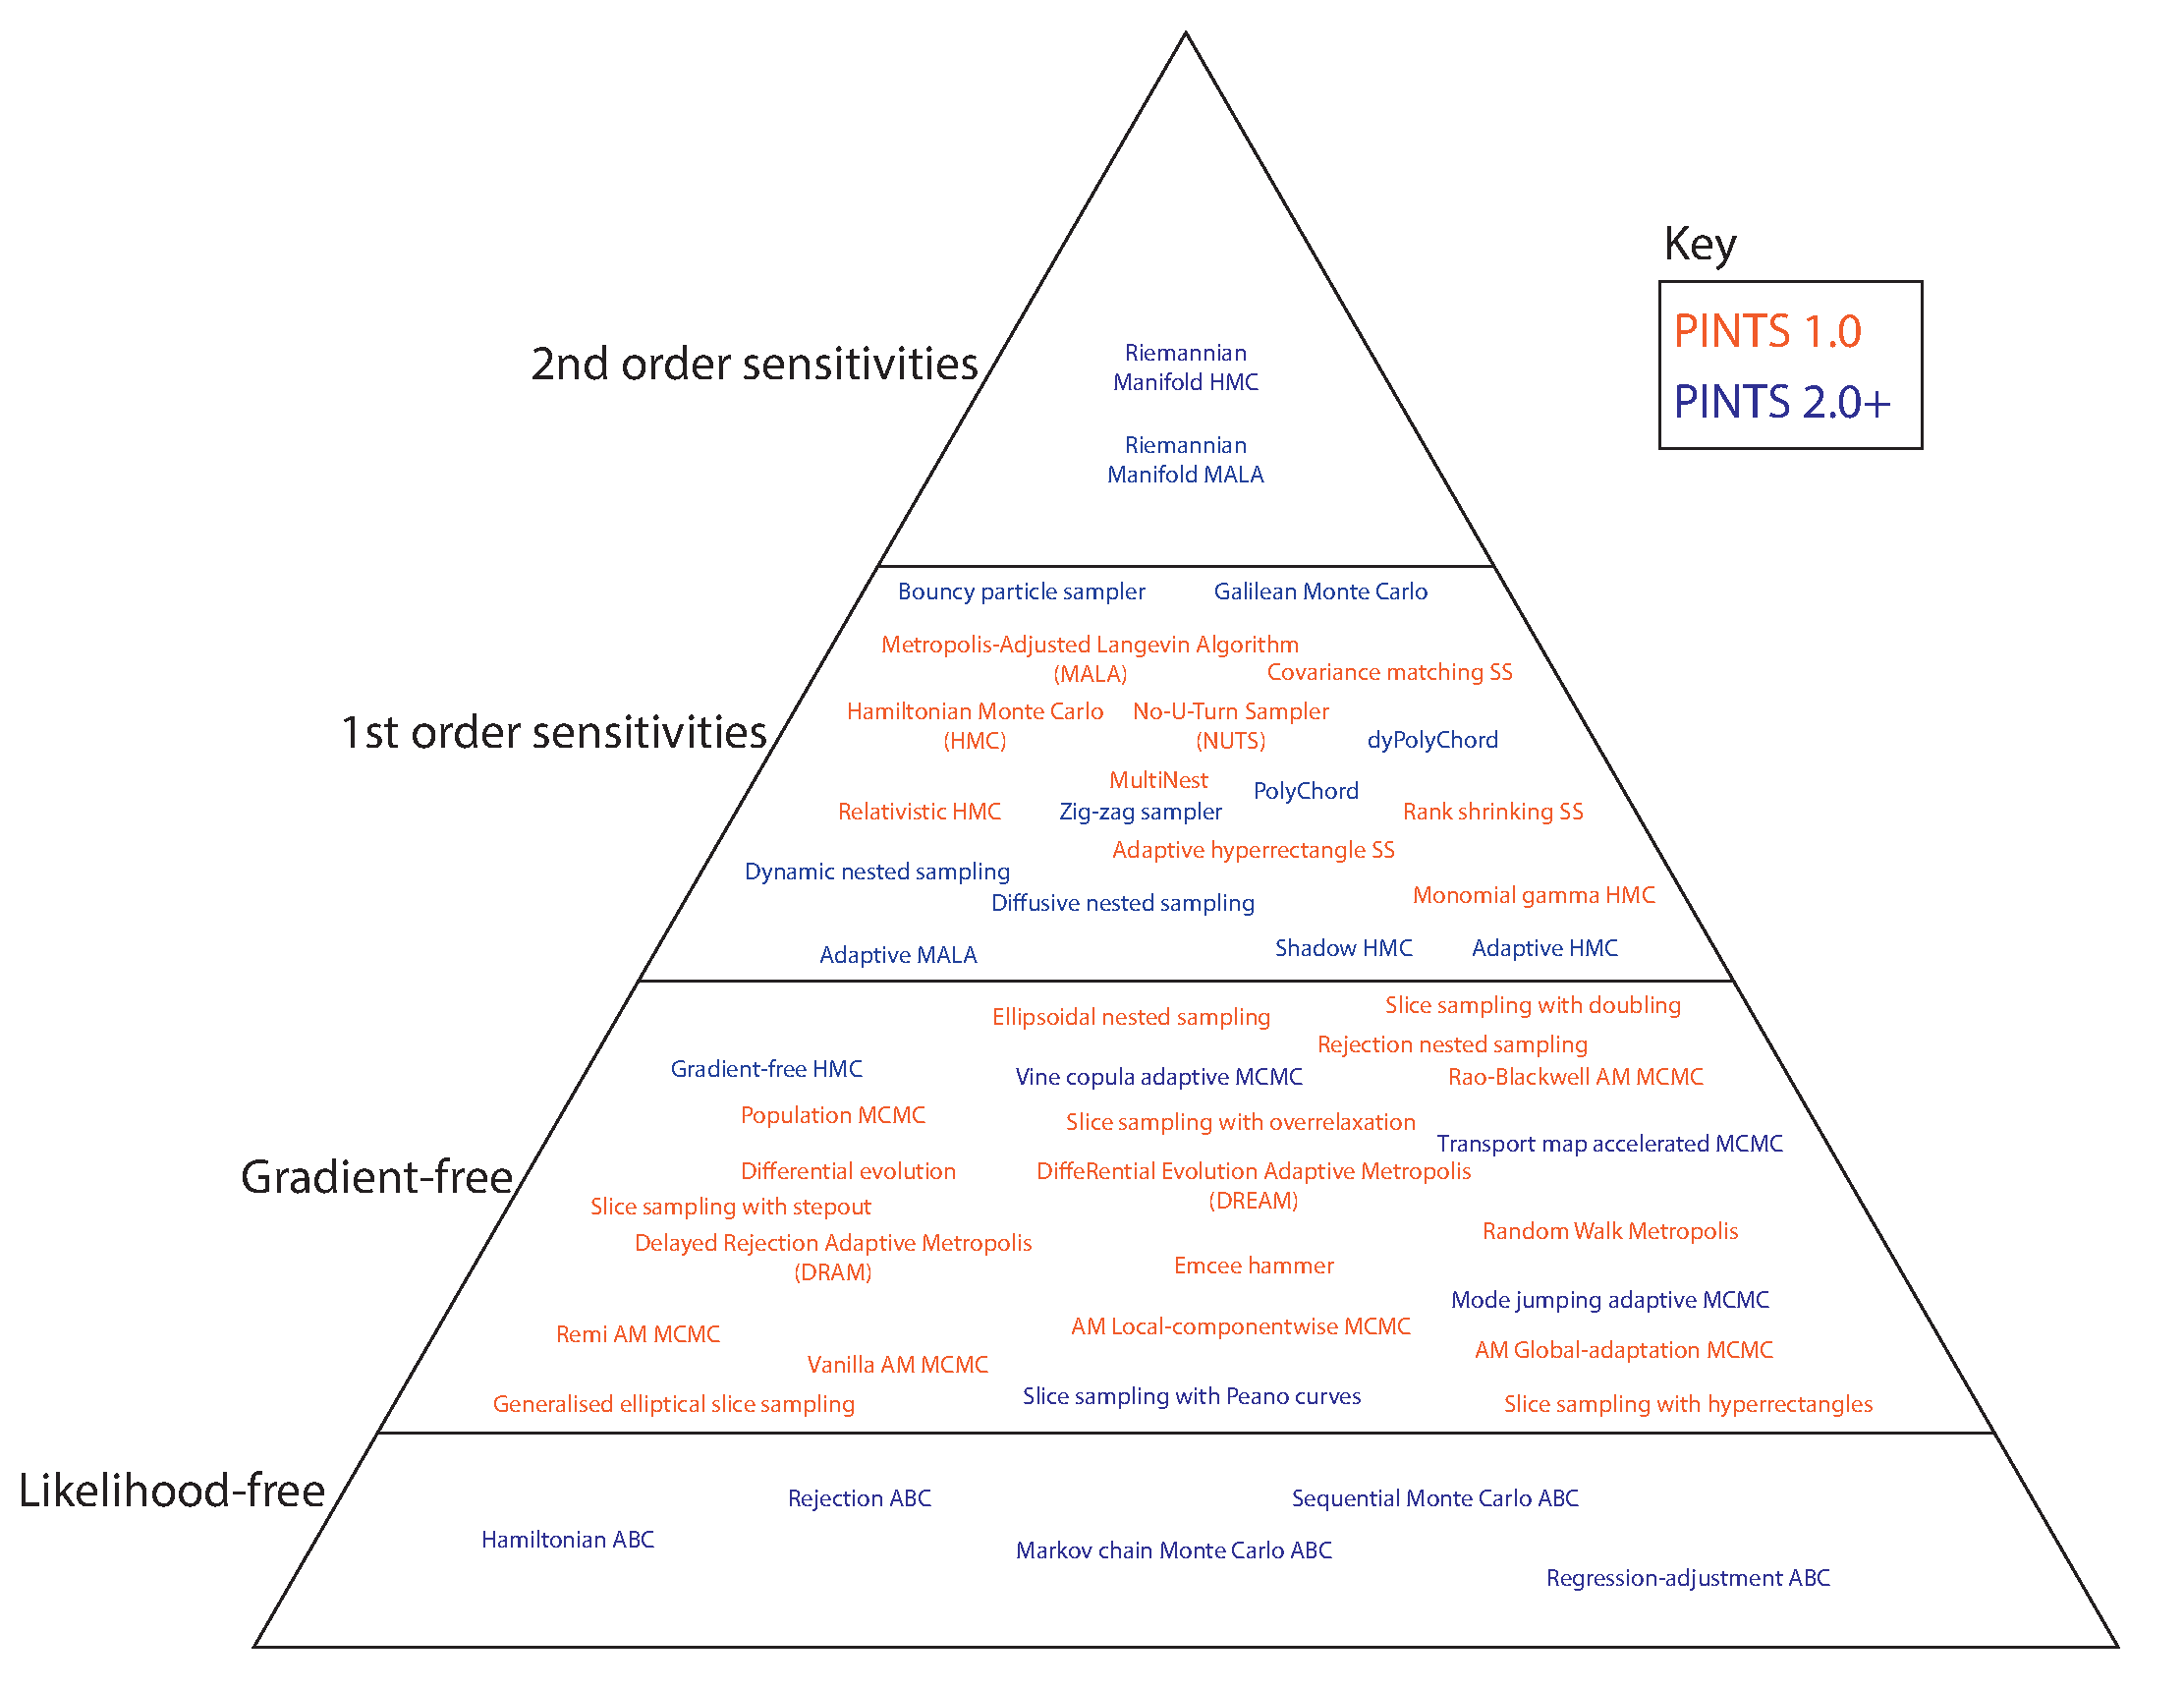
\includegraphics[width=0.9\textwidth]{./Figures/pints-roadmap-triangle-more-samplers.pdf}}
\end{figure}

\end{frame}




\bibliographystyle{authordate1}
\bibliography{Malaria}	 

\end{document}